\documentclass{beamer}


\mode<presentation>
{
  \usetheme{CambridgeUS}
	\usecolortheme{beaver}
  % or ...

  \setbeamercovered{transparent}
  % or whatever (possibly just delete it)
}


\usepackage{xeCJK}
\usepackage[english]{babel}
\usepackage[utf8]{inputenc}
\usepackage{times}
\usepackage[T1]{fontenc}
\usepackage{hyperref}
\usepackage{pifont}
\usepackage{biblatex}
\usepackage{bibentry}
\usepackage{verbatim}
\bibliography{cite}
\newcommand{\cmark}{\ding{51}}%
\newcommand{\xmark}{\ding{55}}%
\setCJKmainfont{WenQuanYi Micro Hei}
\renewcommand{\raggedright}{\leftskip=0pt \rightskip=0pt plus 0cm}
\raggedright

\let\oldfootnotesize\footnotesize
\renewcommand*{\footnotesize}{\oldfootnotesize\tiny}

\title[开源软件基础] 
{开源软件仓库与开源软件生态}
\subtitle{概念与历史}

\author[Zhilei Ren] 
{Zhilei Ren}

\institute[OSCAR Team] % (optional, but mostly needed)
{
\\
\includegraphics[width=0.2\textwidth]{../../utils/logo.jpg}\\
OSCAR Team, School of Software, 
Dalian University of Technology
}


\subject{Open Source}



\pgfdeclareimage[height=0.5cm]{university-logo}{../../utils/logo.jpg}
\logo{\pgfuseimage{university-logo}}



% Delete this, if you do not want the table of contents to pop up at
% the beginning of each subsection:
\AtBeginSubsection[]
{
  \begin{frame}<beamer>{Outline}
    \tableofcontents[currentsection,currentsubsection]
  \end{frame}
}


% If you wish to uncover everything in a step-wise fashion, uncomment
% the following command: 

%\beamerdefaultoverlayspecification{<+->}

\setbeamertemplate{section in toc}[circle]
\setbeamertemplate{items}[circle]
\setbeamertemplate{caption}[numbered]
\setbeamertemplate{bibliography item}{\insertbiblabel}
\setbeamertemplate{bibliography entry title}{}
\setbeamertemplate{bibliography entry journal}{}

\begin{document}

\begin{frame}
  \titlepage
\end{frame}

%\begin{frame}{Outline}
%  \tableofcontents[currentsection,currentsubsection, 
%    hideothersubsections, 
%    sectionstyle=show,
%]
%\end{frame}

\AtBeginSection[]
{
 \begin{frame}<beamer>
 \frametitle{Outline}
 \tableofcontents[currentsection]
 \end{frame}
}
\section{开源软件仓库介绍}
\begin{frame}[t]{软件仓库}
	\begin{block}{定义}
A software repository is a storage location from which software packages may be retrieved and installed on a computer.

Many software publishers and other organizations maintain servers on the Internet for this purpose, either free of charge or for a subscription fee. Repositories may be solely for particular programs, such as CPAN for the Perl programming language, or for an entire operating system\footnote{\url{https://en.wikipedia.org/wiki/Software\_repository}}. 
	\end{block}
\end{frame}

\begin{frame}[t]{典型软件仓库}
	\begin{block}{软件仓库分类}
\begin{itemize}
	\item 操作系统发行版：基于某种内核的操作系统及外围软件构成的完整系统，如Debian、Fedora等GNU/Linux发行版，或FreeBSD、OpenBSD等BSD发行版
	\item 特定语言仓库：提供针对某个语言的软件包/类库等，如Perl的CPAN、R的CRAN、\TeX{}的CTAN、C++的boost等
\end{itemize}
	\end{block}
\end{frame}

\begin{frame}[t]{软件仓库}
	\begin{block}{软件仓库的操作}
Operators of such repositories typically provide a package management system, tools intended to search for, install and otherwise manipulate software packages from the repositories. For example, many Linux distributions use Advanced Packaging Tool (APT), commonly found in Debian based distributions, or yum found in Red Hat based distributions. There are also multiple independent package management systems, such as pacman, used in Arch Linux and equo, found in Sabayon Linux.
	\end{block}
\end{frame}
\begin{frame}[t,fragile]{APT梗}
	\begin{block}{今天就能开始用的小知识}
	\scriptsize
	\begin{verbatim}
$apt moo
                 (__) 
                 (oo) 
           /------\/ 
          / |    ||   
         *  /\---/\ 
            ~~   ~~   
..."Have you mooed today?"...
$ LC_ALL=C apt |tail -n 1
                                        This APT has Super Cow Powers.
$ apt |tail -n 1
                                         本 APT 具有超级牛力。
\end{verbatim}
\end{block}
\end{frame}
\begin{frame}[t]{Linux发行版}
	\centering
	placeholder for timeline
	%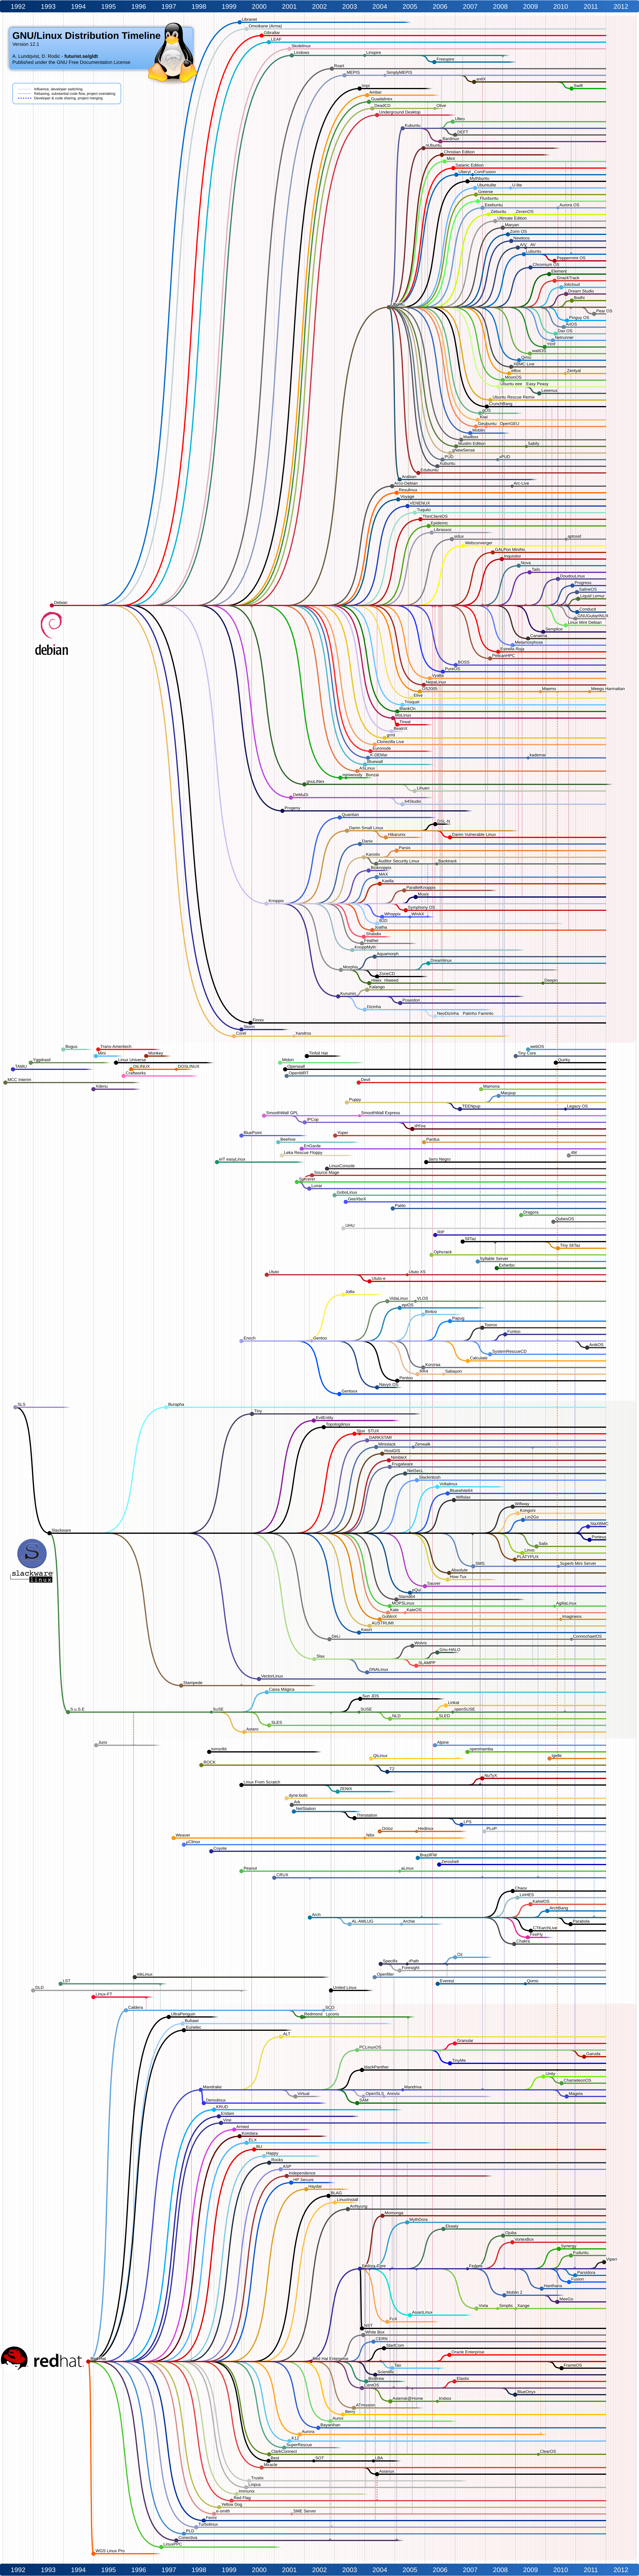
\includegraphics[width=0.25\textwidth,angle=90]{distro-timeline.png}
\end{frame}
\begin{frame}[t]{典型Linux发行版}
	\begin{block}{Debian}
		Debian是完全由自由软件组成的类UNIX操作系统，其包含的多数软件使用GNU通用公共许可协议授权，并由Debian计划的参与者组成团队对其进行打包、开发与维护。

Debian项目最初由伊恩·默多克于1993年发起，Debian 0.01版在1993年9月15日发布，而其第一个稳定版本则在1996年发布。\footnote{\url{https://zh.wikipedia.org/zh-cn/Debian}}

	\end{block}
		\centering
		
\includegraphics[width=0.4\textwidth]{debian.png}
\end{frame}
\begin{frame}[t]{典型Linux发行版}
	\begin{block}{Debian的特色}
Debian以其坚守Unix和自由软件的精神，以及其给予用户的众多选择而闻名。现时Debian提供了超过25,000个软件，超过50,000个软件包，并正式支持10个计算机系统结构。

作为一个大的系统组织框架，Debian旗下有多种不同操作系统核心的分支计划，主要为采用Linux核心的Debian GNU/Linux系统，其他还有采用GNU Hurd核心的Debian GNU/Hurd系统、采用FreeBSD核心的Debian GNU/kFreeBSD系统等。众多知名的Linux发行版，例如Ubuntu、Knoppix和Deepin，也都建基于Debian GNU/Linux。

	\end{block}
\end{frame}
\begin{frame}[t]{典型Linux发行版}
	\begin{block}{今天就能开始用的小知识}
		\begin{itemize}
			\item Debian名字来源于发起人Ian Murdock和当时的女友Debra Lynn
			\item Debian的版本号昵称来自玩具总动员
			\item Debian的logo来自玩具总动员角色巴斯光年的胡子（存疑）%\footfullcite{krafft2005debian}
		\end{itemize}
\end{block}
\begin{minipage}{.5\textwidth}
	\centering
	
\includegraphics[width=0.4\textwidth]{buzz.jpg}
\end{minipage}
\begin{minipage}{.5\textwidth}
	\centering
	
\includegraphics[width=0.2\textwidth]{officiallogo-100.jpg}
\end{minipage}
\end{frame}
\begin{frame}[t]{Debian}
	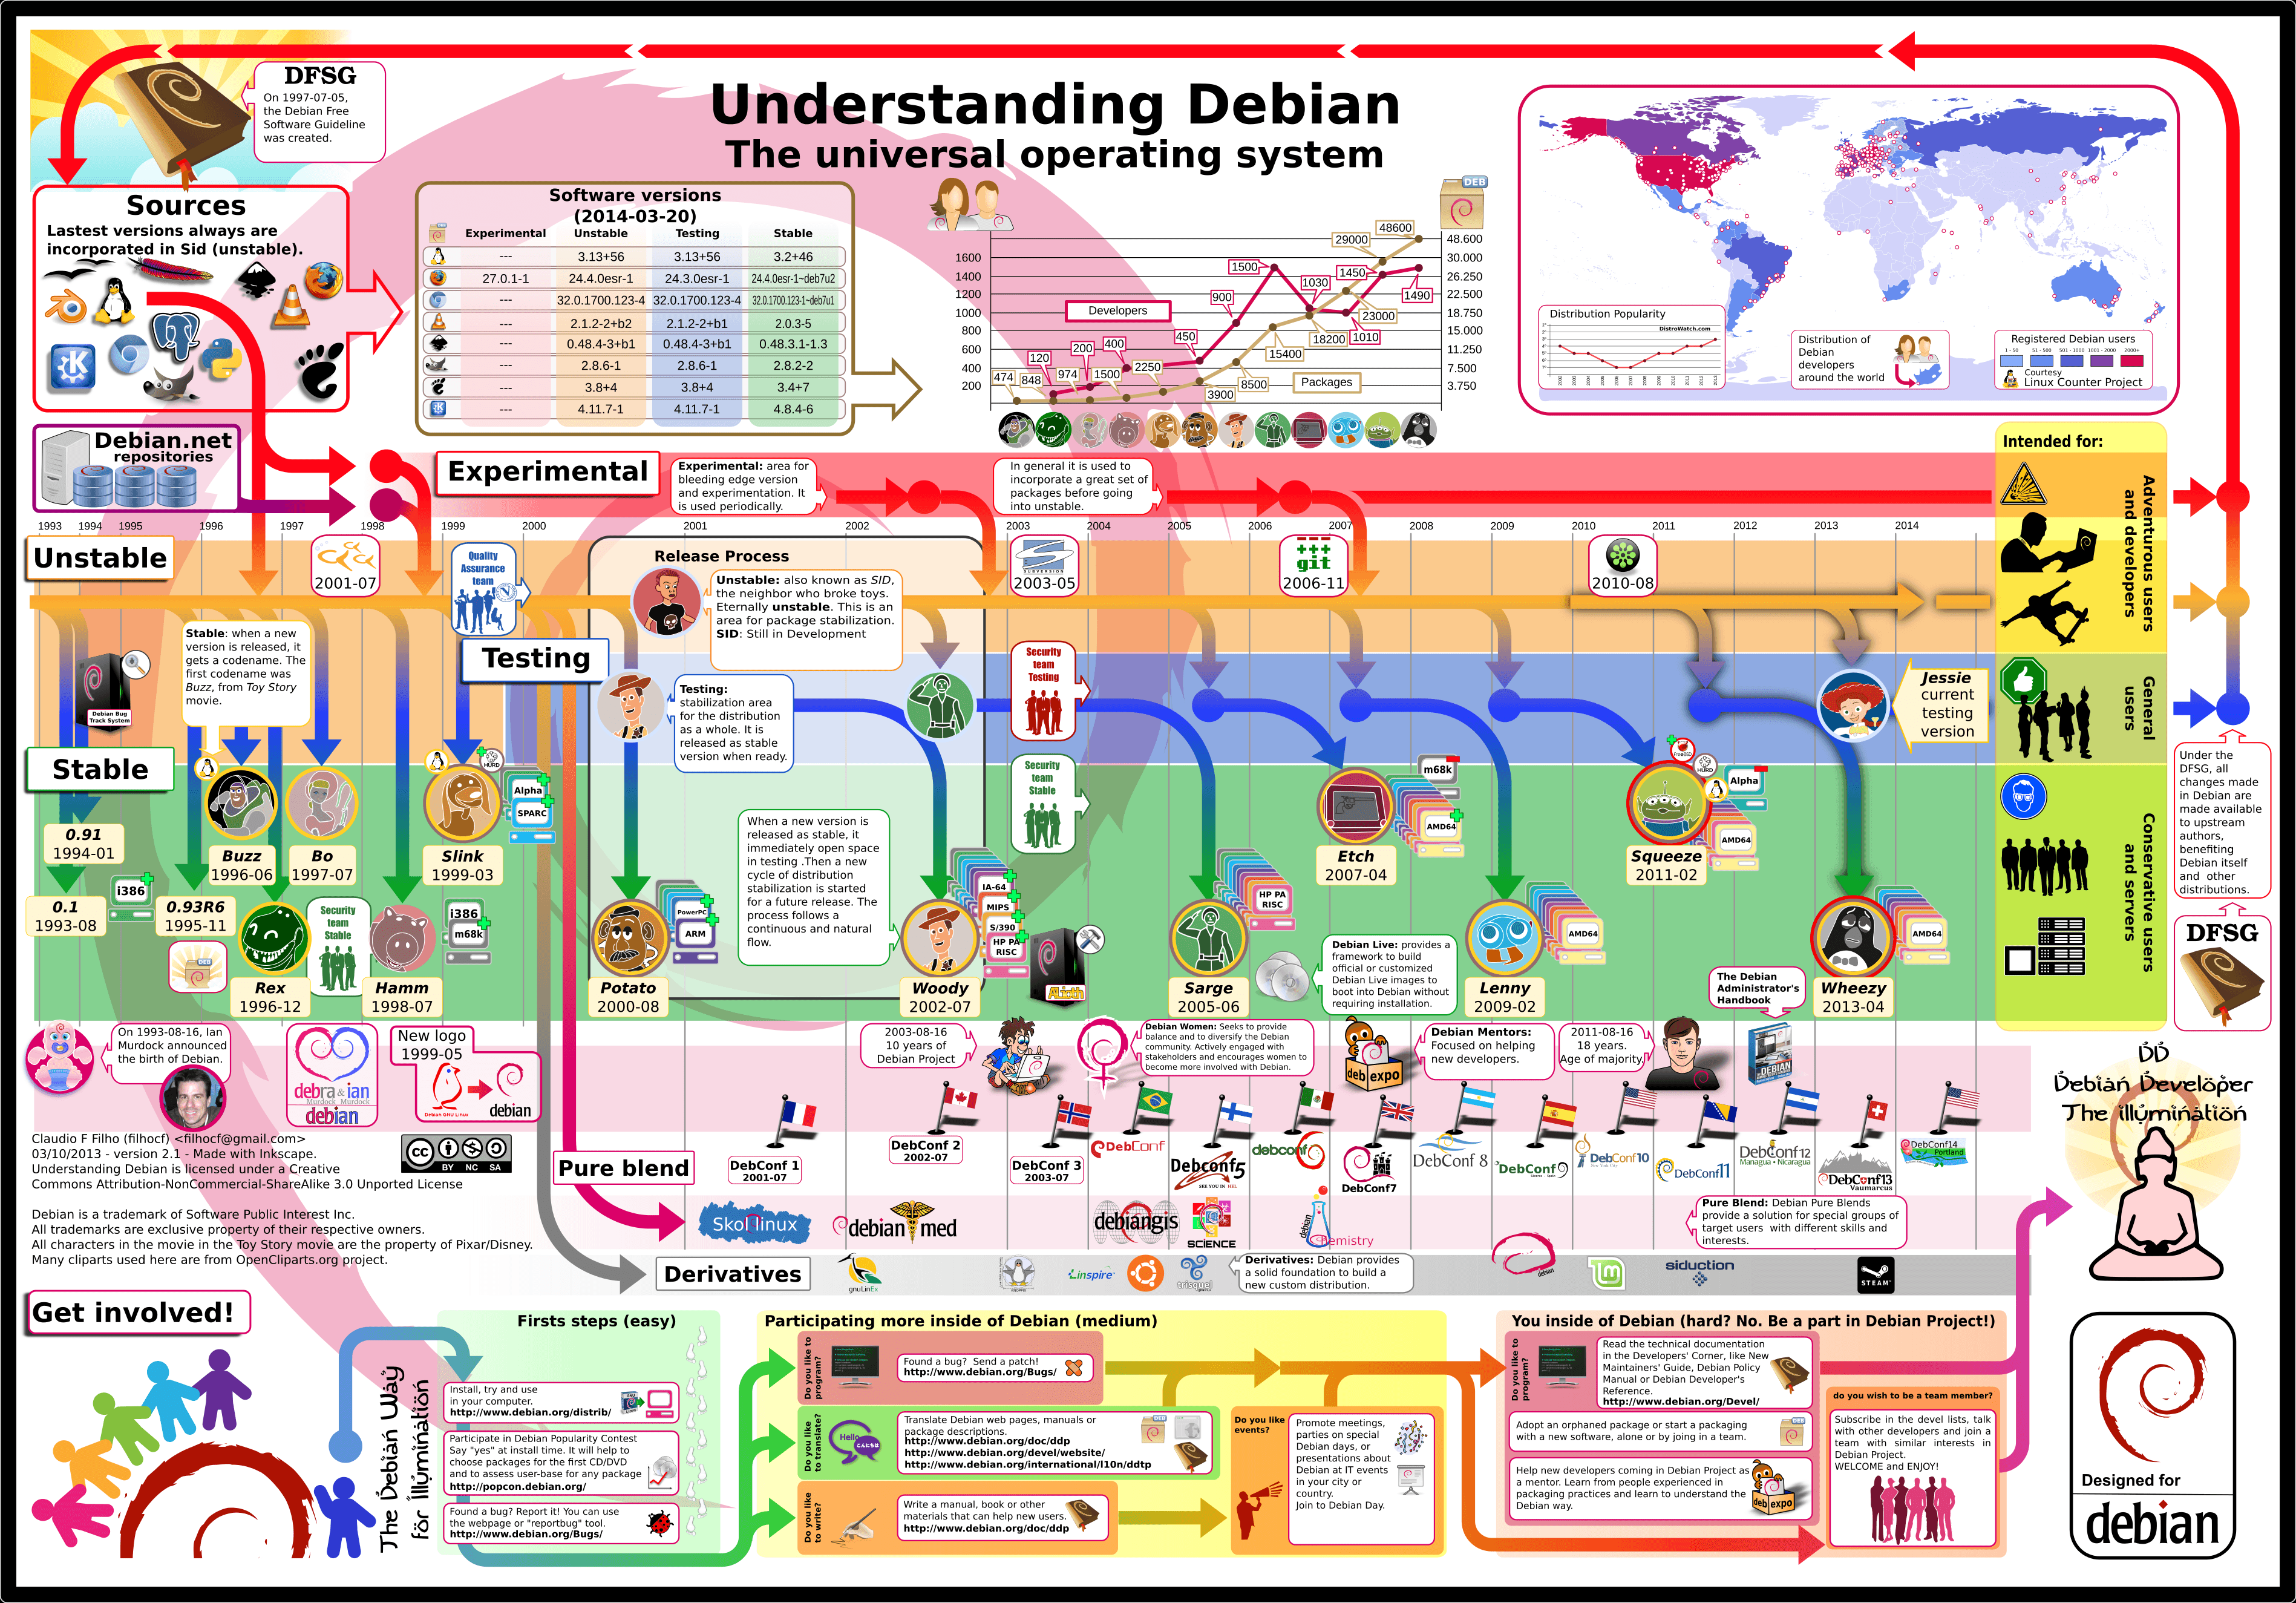
\includegraphics[width=0.9\textwidth]{understanding-debian.png}
\end{frame}
\begin{frame}[t]{典型Linux发行版}
	\begin{block}{Ubuntu}
		\begin{itemize}
			\item Ubuntu是以桌面应用为主的Linux发行版，Ubuntu由Canonical公司发布，他们提供商业支持。它是基于自由软件，其名称来自非洲南部祖鲁语或科萨语的ubuntu一词，意思是``人性''、``我的存在是因为大家的存在''，是非洲传统的一种价值观。
			\item Ubuntu在Ubuntu 12.04的发布页面上使用了``友帮拓''作为官方译名。
		\end{itemize}
	\end{block}
		\centering
		
\includegraphics[width=0.25\textwidth]{ubuntu.png}
\end{frame}
\begin{frame}[t]{Ubuntu}
	\begin{block}
		{今天就能开始使用的小知识}
		Ubuntu的发行代码规律

		\scriptsize
		\begin{tabular}{lll}
4.10     	&  Warty Warthog         	&  多疣的疣猪         	\\
5.04     	&  Hoary Hedgehog        	&  白发的刺猬         	\\
5.10     	&  Breezy Badger         	&  活泼的獾           	\\
6.06LTS  	&  Dapper Drake          	&  整洁的公鸭         	\\
6.10     	&  Edgy Eft              	&  尖利的小蜥蜴       	\\
7.04     	&  Feisty Fawn           	&  烦躁不安的鹿       	\\
7.10     	&  Gutsy Gibbon          	&  胆大的长臂猿       	\\
8.04LTS  	&  Hardy Heron           	&  坚强的鹭           	\\
8.10     	&  Intrepid Ibex         	&  无畏的羱羊         	\\
9.04     	&  Jaunty Jackalope      	&  活泼的鹿角兔       	\\
9.10     	&  Karmic Koala          	&  幸运的树袋熊       	\\
10.04LTS 	&  Lucid Lynx            	&  清醒的山猫         	\\
\end{tabular}
\end{block}
\end{frame}
\begin{frame}[t]{Ubuntu}
	\begin{block}
		{今天就能开始使用的小知识}
		Ubuntu的发行代码规律

		\scriptsize
		\begin{tabular}{lll}
10.10    	&  Maverick Meerkat      	&  标新立异的狐獴     	\\
11.04    	&  Natty Narwhal         	&  敏捷的独角鲸       	\\
11.10    	&  Oneiric Ocelot        	&  有梦的虎猫         	\\
12.04LTS 	&  Precise Pangolin      	&  精准的穿山甲       	\\
12.10    	&  Quantal Quetzal       	&  量子的格查尔鸟     	\\
13.04    	&  Raring Ringtail       	&  铆足了劲的环尾猫熊 	\\
13.10    	&  Saucy Salamander      	&  活泼的蝾螈         	\\
14.04LTS 	&  Trusty Tahr           	&  可靠的塔尔羊       	\\
14.10    	&  Utopic Unicorn        	&  乌托邦的独角兽     	\\
15.04    	&  Vivid Vervet          	&  活泼的长尾黑颚猴   	\\
15.10    	&  Wily Werewolf         	&  老谋深算的狼人     	\\
16.04LTS 	&  Xenial Xerus          	&  好客的非洲地松鼠   	\\
16.10    	&  Yakkety Yak           	&  喋喋不休的牦牛     	\\
17.04    	&  Zesty Zapus           	&  热情的美洲林跳鼠   	\\
17.10    	&  Artful Aardvark       	&  巧妙的土豚         	\\
18.04LTS 	&  Bionic Beaver         	&  仿生的海狸         	\\
			
		\end{tabular}
	\end{block}
	
\end{frame}
\begin{frame}[t]{典型Linux发行版}
	\begin{block}{ArchLinux}
	\end{block}
		\centering
		
\includegraphics[width=0.25\textwidth]{archlinux.png}
\end{frame}
\begin{frame}[t]{典型Linux发行版}
	\begin{block}{Red Hat}

	\end{block}
		\centering
		
\includegraphics[width=0.25\textwidth]{redhat.jpg}
\end{frame}
\begin{frame}[t]{典型Linux发行版}
	\begin{block}{Fedora}

	\end{block}
		\centering
		
\includegraphics[width=0.25\textwidth]{fedora.jpg}
\end{frame}
\begin{frame}[t]{典型Linux发行版}
	\begin{block}{Gentoo}

	\end{block}
		\centering
		
\includegraphics[width=0.25\textwidth]{gentoo.png}
\end{frame}
\begin{frame}[t]{特定语言仓库}
	\begin{block}{Pypi}
		\url{http://kgullikson88.github.io/blog/pypi-analysis.html}
	\end{block}
	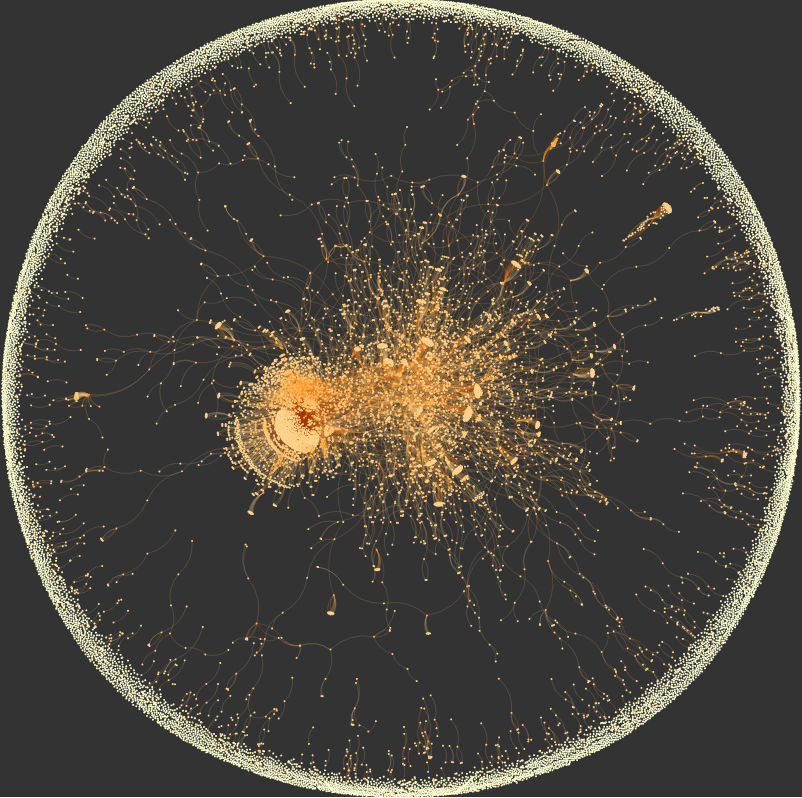
\includegraphics[width=0.8\textwidth]{pypi2.png}
\end{frame}
\begin{frame}[t]{特定语言仓库}
	\begin{block}{CRAN}
		Knowledge Flows in Open Source Software Supply Chains
		NASAC 2017 Keynote Audris Mockus
	\end{block}
	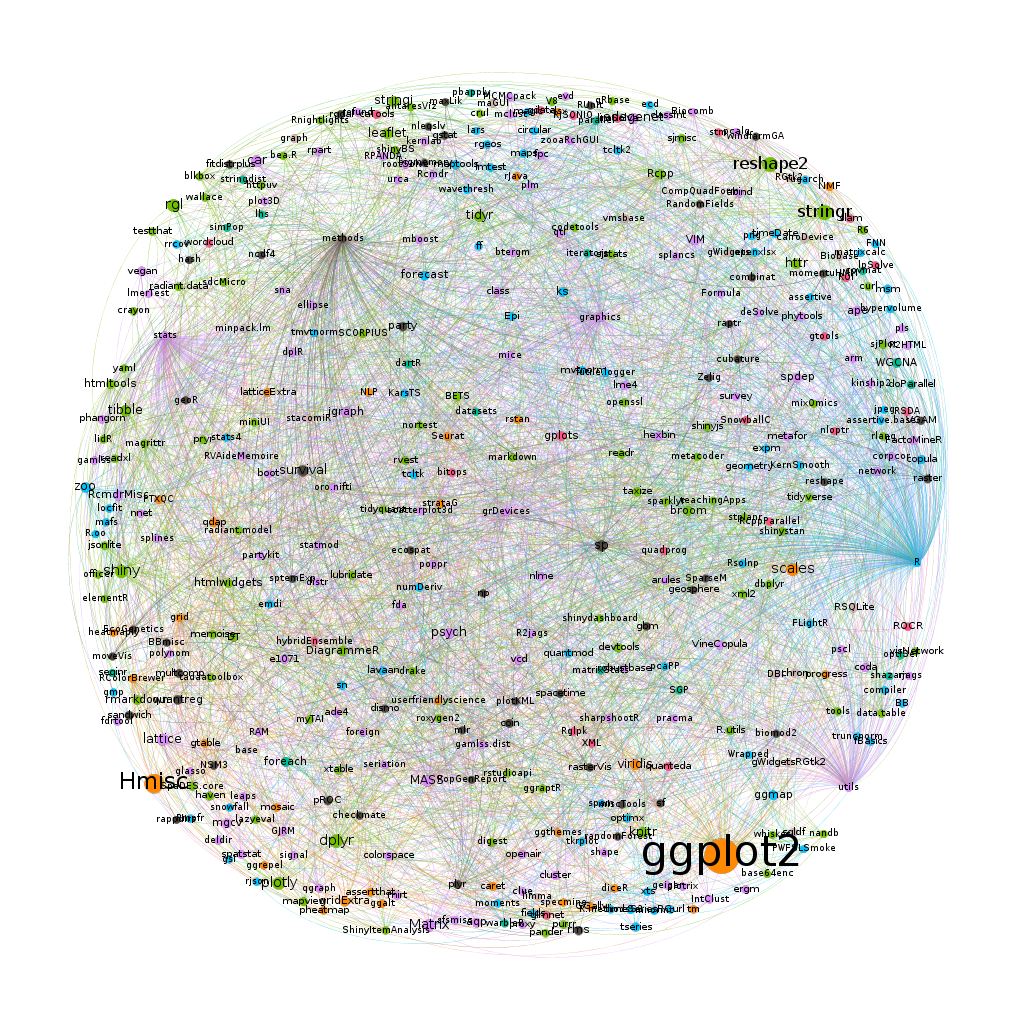
\includegraphics[width=0.8\textwidth]{r.png}
\end{frame}
\begin{frame}[t]{特定语言仓库}
	\begin{block}{CPAN}
\url{http://mapofcpan.org/}
	\end{block}
	\centering
	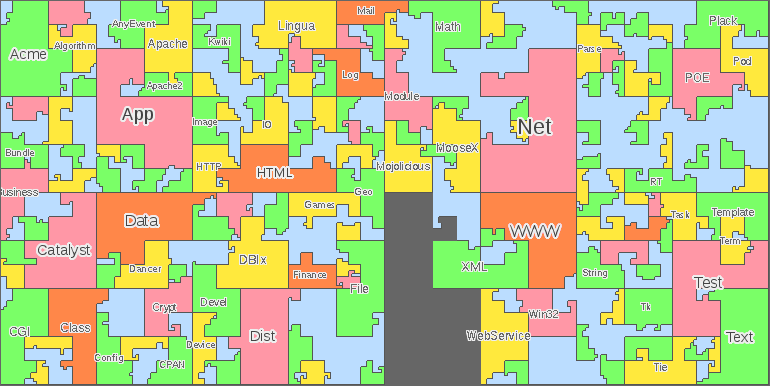
\includegraphics[width=0.8\textwidth]{map-of-cpan.png}
\end{frame}
\section{开源软件仓库结构}
\begin{frame}[t]{以Debian为例}
	\begin{block}{Debian的基本结构}

	\end{block}
	
\end{frame}

\begin{frame}[t]{以Debian为例}
	\begin{block}{Debian社会契约}

	\end{block}
	
\end{frame}
\begin{frame}[t]{以Debian为例}
	\begin{block}{Debian的发布周期}

	\end{block}
	
\end{frame}
\begin{frame}[t]{以Debian为例}
	\begin{block}{Debian的发布流程}

	\end{block}
	
\end{frame}
\begin{frame}[t,fragile]{以Debian为例}
	\begin{block}{Debian的依赖管理}
		\scriptsize
		\begin{verbatim}
$debtree nano | dot -Tpng > nano.png
digraph "nano" {
  rankdir=LR;
  node [shape=box];
  "nano" -> "libncursesw5" [color=blue,label="(>= 6)"];
  "libncursesw5" -> "libtinfo5" [color=blue,label="(= 6.0+20170902-1)"];
  "libncursesw5" -> "libgpm2";
  "nano" -> "libtinfo5" [color=blue,label="(>= 6)"];
  "nano" -> "pico" [color=red];
  "nano" [style="setlinewidth(2)"]
  "pico" [style=filled,fillcolor=oldlace];
}
// Excluded dependencies:
// libc6 zlib1g
// total size of all shown packages: 3093504
// download size of all shown packages: 976236
\end{verbatim}
	\end{block}
	
\end{frame}
\begin{frame}[t,fragile]{以Debian为例}
	\begin{minipage}{0.5\textwidth}
		\scriptsize
\begin{verbatim}
Package: nano
Priority: standard
Section: editors
Installed-Size: 716
Architecture: amd64
Version: 2.6.3-1
Replaces: pico
Provides: editor
Depends: libc6 (>= 2.14), libncursesw5 (>= 6), libtinfo5 (>= 6)
Suggests: spell
Conflicts: pico
Description-en: small, friendly text editor inspired by Pico
 GNU nano is an easy-to-use text editor originally designed 
 as a replacement for Pico, the ncurses-based editor from 
the non-free mailer package Pine (itself now available under 
the Apache License as Alpine).
\end{verbatim}
	\end{minipage}
	\begin{minipage}{0.5\textwidth}
		\vspace{-1in}
	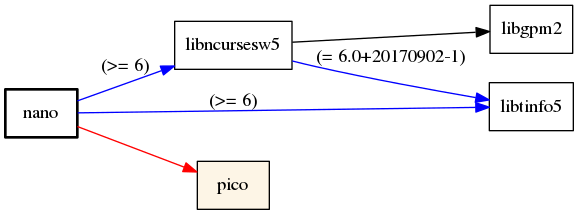
\includegraphics[width=0.8\textwidth]{nano.png}
	\end{minipage}
	
\end{frame}
\begin{frame}[t]{以Debian为例}
	placeholder for vim
	%\includegraphics[width=0.8\textwidth]{vim.png}
	
\end{frame}
\begin{frame}[t]{以Debian为例}
	\begin{block}{Debian的Bug管理}

	\end{block}
	
\end{frame}
\begin{frame}[t]{以Debian为例}
	\begin{block}{Debian的基本结构}

	\end{block}
	
\end{frame}
\end{document}
